\documentclass[12pt, letterpaper]{article}
\usepackage[utf8]{inputenc}
\usepackage{indentfirst}
\usepackage{graphicx}
\usepackage{setspace}
\usepackage[numbers]{natbib}
\usepackage [autostyle, english = american]{csquotes}
\MakeOuterQuote{"}
\usepackage{layout}
\usepackage[title]{appendix}
\usepackage[justification=centering]{caption}
\usepackage{titlesec}
\usepackage[percent]{overpic}
\usepackage{amsmath}
\usepackage{systeme}
\usepackage{blkarray, bigstrut}
\usepackage{tikz}
\usetikzlibrary{tikzmark}
\usepackage[utf8]{inputenc}
\usepackage{relsize}
\usepackage[nameinlink, capitalize, noabbrev]{cleveref}
\usepackage{tabu}

\setlength\parskip{\baselineskip}

%prevent hyphenation of words
%\emergencystretch=\maxdimen
\hyphenpenalty=10000
%\hbadness=10000

\begin{document}

\setcounter{secnumdepth}{-1}
\titlespacing*{\section}{0pt}{1.5\baselineskip}{.25\baselineskip}
\binoppenalty=\maxdimen
\relpenalty=\maxdimen

\setlength{\abovedisplayskip}{-0.5\baselineskip}
\setlength{\belowdisplayskip}{0\baselineskip}
\setlength{\abovedisplayshortskip}{0\baselineskip}
\setlength{\belowdisplayshortskip}{0\baselineskip}

%Cover page: 5pts
%Course, subject, name, date
\title{MA348 Numerical Analysis, Integration}
\author{David Jefts}
\date{April 24\textsuperscript{th}, 2019}
\begin{titlepage}
	\centering
	\maketitle
	\centering
	\hfill
	\vfill
	\thispagestyle{empty}
\end{titlepage}

\setlength{\voffset}{-0.5in}
\setlength{\headsep}{10pt}

%Introduction: 5pts
%Describe the problem and state objectives
\section{\label{sec:intro}Introduction}
	%Lab9: Use the trapezoid rule ( with 2, 4 and 6 intervals) , the Simpson rule( with 5 points) and the Gaussian quadrature with 2 points to approximate : the integral of f between 0 and 0.8, where f(x)=0.2+25x-200x^2+675x^3-900x^4+400x^5
	The purpose of this lab is to use compare the effectiveness of different algorithms at estimating the value of an integral, $\displaystyle\int_{a}^{b}\!{f(x)}\,\mathrm{d}x$, where $a$ is 0, $b$ is 0.8, and $f(x)={0.2+25x-200x^2+675x^3-900x^4+400x^5}$.
	
	$\displaystyle\int_{0.0}^{0.8}\!{0.2+25x-200x^2+675x^3-900x^4+400x^5}\,\mathrm{d}x$
	 
	 The two methods used to solve the above definite integral were the Newton-Cotes Trapezoidal Method and the Newton-Cotes Simpson method. The Trapezoid method was used with 2-, 4-, and 6-subintervals, while the Simpson method was used with five subintervals.

%Theory-Analysis: 5pts
%State assumptions and develop equations
\section{\label{sec:theory}Theory-Analysis}
	The Newton-Cotes Trapezoidal method is an integration method based on splitting up an integral into $n$ subintervals, drawing a straight line between each pair of $f(x_n)$ and $f(x_{n+1}$ values to create a series of trapezoids. These trapezoids can then be used to estimate the integral value of the function. The area of a trapezoid can be represented by the function $A=\frac{h}{2}left(a+b)$ where h is the width of the trapezoid, $a$ is the height of the left trapezoid edge, and $b$ is the height of the right trapezoid edge. The fourth edge of the trapezoid is not needed to find the area. By replacing $a$ with $x_i$ and $b$ with $x_{i+1}$ then creating a summation from $i=0$ to $i=n$, the function can be rewritten as:
	
	\begin{equation*} I = \frac{h}{2} \left[f(x_0)+2\sum_{i=1}^{n-1}{f(x_i)}+f(x_n)\right] \end{equation*}
	
	The middle sum term of the bracketed equation is multiplied by two because each subinterval's $y$-value will be used twice, except for the first and last points.
	
	Simpson's integral estimation equation is an extension of the Newton-Cotes method, but adds the midpoint of each subinterval into the estimation function to make the estimate more accurate by using three points on each subinterval instead of two. It uses a Lagrange polynomial interpolation to generate a standard second-degree curve along these three points and then estimates the area. The function for this interpolated line is much more complicated than the trapezoid area function:
	
	\begin{equation*} y_i = f(x_i) \frac{(x-x_{i+1})(x-x_{i+2})}{(x_i-x_{i+1})(x_i-x_{i+2})} + 
		f(x_{i+1}) \frac{(x-x_{i+1})(x-x_{i+2})}{(x_{i+1}-x_i)(x_{i+1}-x_{i+2})} + 
	\end{equation*}\begin{equation*}
		f(x_{i+2}) \frac{(x-x_{i+1})(x-x_{i+2})}{(x_{i+2}-x_i)(x_{i+2}-x_{i+1})}
	\end{equation*}
	
	When summed from $i=0$ to $i=n$, the equation is simplified to:
	
	\begin{equation*} I = \frac{h}{3} \left[f(x_0)+4\!\!\!\sum_{i=1, 3, 5...}^{n-1}{\!\!\!f(x_i)}+2\!\!\!\sum_{i=2, 4, 6...}^{n-1}{\!\!\!f(x_i)}+f(x_n)\right] \end{equation*}
	
	For the purpose of testing it was assumed that the actual value of the integral is 1.640533333.

	 
%Numerical Solution: 20pts
%Describe the numerical methods used to solve the problem
\section{\label{solution}Numerical Solution}
	All three integration methods were coded in Python, with this report created in \LaTeX{}.
	
	The Newton-Cotes Trapezoidal method is a method of integration based upon breaking up the integral into multiple subintervals and then drawing trapezoids that estimate the area under the function curve, as shown below:
	
	\begin{figure}[h]
            		\centering
            		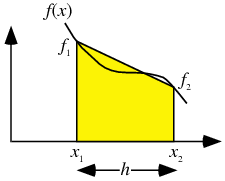
\includegraphics[width=0.5\linewidth]{trapezoid.png}
            	\end{figure}
	
	 \newpage$f(x)$ is the function line, $h$ is the width of each subinterval (also known as the $\delta x$), $x_1$ and $x_2$ are the endpoints of the subinterval and $f_1$ and $f_2$ are the corresponding function values. The yellow area is the trapezoid that represents the integral estimation for that subinterval and is represented by:
	 
	 \begin{equation*} I = \frac{h}{2} \left[f(x_0)+2\sum_{i=1}^{n-1}{f(x_i)}+f(x_n)\right] \end{equation*}
	 
	 This is a summation of all of the trapezoids between each limit of the integral when there is $n$ subintervals with each $x$ value representing the vertical lines dividing the subintervals. $h$ is equivalent to $a$
	 
	 The Simpson formula is very similar to the Trapezoidal formula, except that it uses the midpoint of each subinterval as well as the end points when estimating the integral value.
	 
	 \begin{equation*} I = \frac{h}{3} \left[f(x_0)+4\!\!\!\sum_{i=1, 3, 5...}^{n-1}{\!\!\!f(x_i)}+2\!\!\!\sum_{i=2, 4, 6...}^{n-1}{\!\!\!f(x_i)}+f(x_n)\right] \end{equation*}


%Results and Discussion: 45pts
%Tabulate and plot the results, compare results, and discuss the accuracy of results
\section{\label{sec:results}Results and Discussion}
    	The table depicting the various integral values is shown below:
	
	\begin{table}[h]
	\centering
	\begin{tabular}{l | >{$}c<{$} | >{$}c<{$}}
	\textbf{Method} & \textbf{Value} & \textbf{Percentage Error} \\\hline
	By-Hand Integration & 1.6405333333333333 & 0.0000\% \\\hline
	Trapezoid Rule (2 points) & 0.5312000000000001 & 67.620\% \\
	Trapezoid Rule (4 points) & 0.6240000000000006 & 61.964\% \\
	Trapezoid Rule (6 points) & 0.8981816186556900 & 45.251\% \\
	Trapezoid Rule (8 points) & 1.1246500000000006 & 31.446\% \\\hline
	Simpson Rule (4 points) & 0.587733333333333 & 64.174\% \\
	Simpson Rule (6 points) & 0.9335601280292622 & 43.094\% \\
	Simpson Rule (8 points) & 1.1645000000000005 & 29.017\% \\
	\end{tabular}
	\end{table}
	
	Based on these results, the Simpson Method converges faster and generally has a lower error when using a similar amount of points as the Trapezoid Rule. However, the error for the Simpson method increases by 20-30\% when there is an odd number of points, so on average the Trapezoid Rule is more effective. However when the number of points is predetermined to be even then the Simpson Method will be more accurate.
	


%Conclusions: 20pts
%Comment on the efficiency of the solvers
\section{\label{conclusion}Conclusions}
	Both the Simpson Method and the Trapezoid Rule are very effective at estimating definite integral functions but the Simpson Method routinely resulted in more accurate integrals. To contrast that, the Trapezoidal Rule was considerably easier to implement and works correctly regardless of the number of subintervals, while the Simpson Method requires an even number of points to produce an accurate measurement. In conclusion, the Simpson Method is more accurate, but only when the number of subintervals is even. 

\pagebreak
%Appendices
%Include listings of the source codes, include printed copies of the output files
\appendix
	\section{Appendix A}
            	\begin{figure}[h]
            		\centering
            		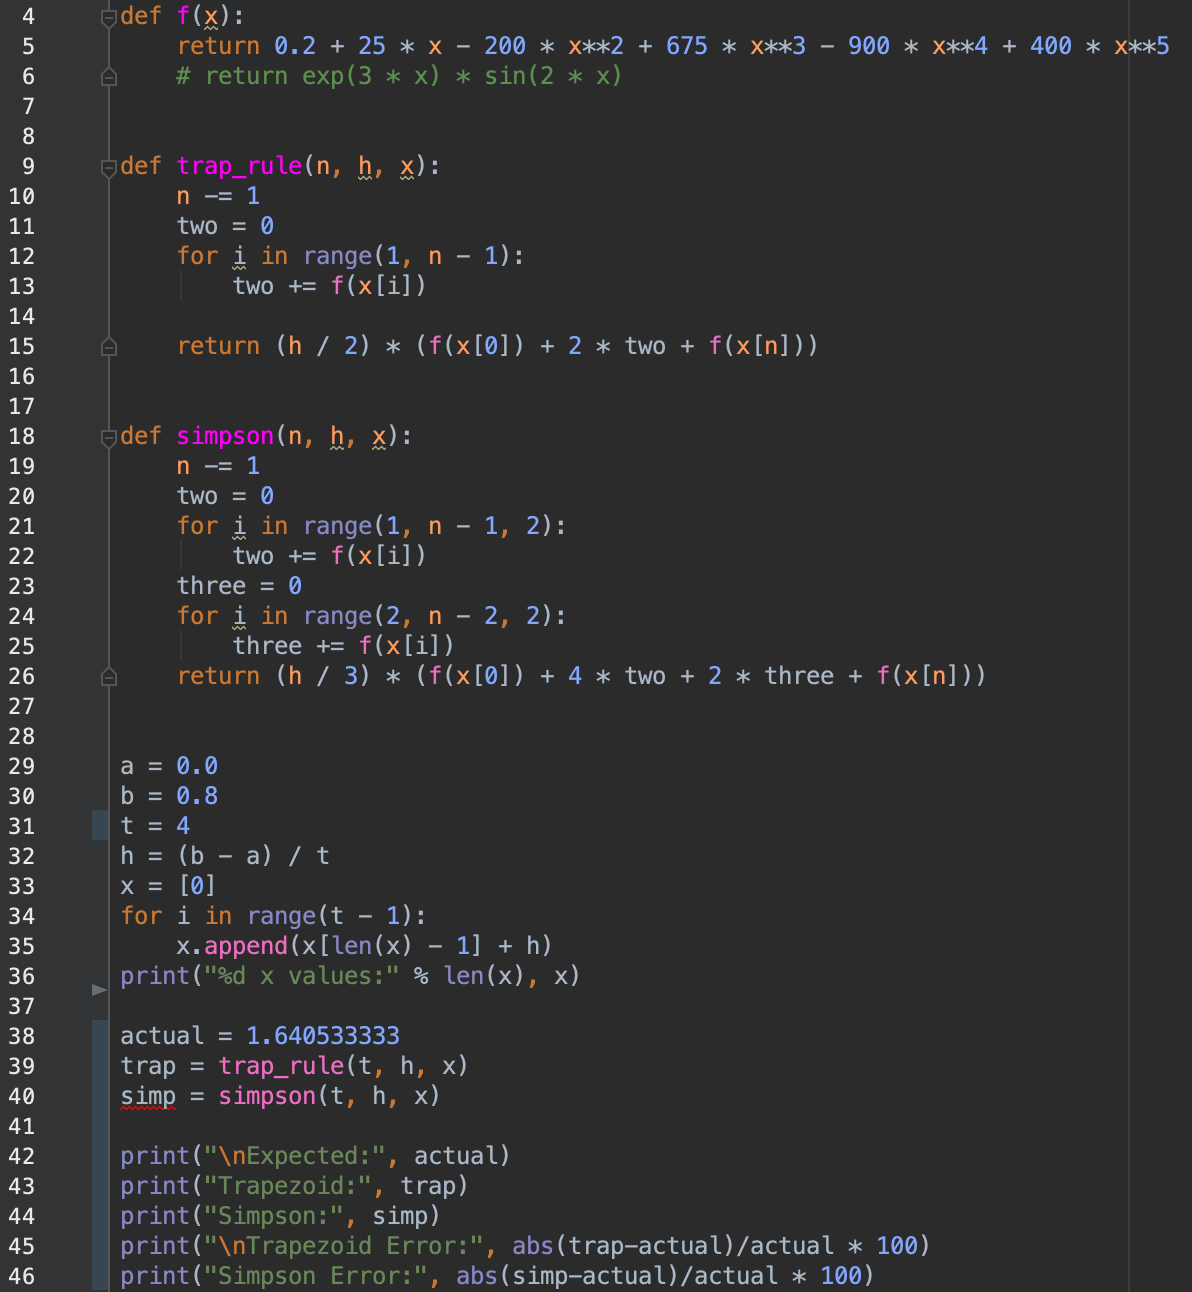
\includegraphics[width=1.0\linewidth]{PythonCode.png}
            	\end{figure}
		
		
		


\end{document}
